\chapter{Simulation and Development}
\label{ch:sim}
The simulation and development of the BONuS12 experiment has been ongoing essentially since the original BONuS6 experiment in the early 2000's. The goal of BONuS has always been to detect low momentum spectator protons in coincidence with scattered electrons at high Bjoken-x. This is the purpose of the simulation and development (\textit{i.e.} to optimize a detector that will result in high statistics in the relevant kinematic range).

This chapter will focus on the methods used in that detector optimization in preparation for the BONuS12 experimental run. It will cover simulations done to improve geometry, determine  electron drift time, and understand energy loss through detector components. The chapter will also go over the construction of the detector. Finally, the process of reconstruction will be covered, which is the way we ultimately determine the kinematics of each event in order to recover the structure functions we are interested in.

\section{Geant4 Monte Carlo (GEMC)}
Much of the simulations done in preparation for and during CLAS12 experiments use the Geant4 Monte Carlo (GEMC) software developed by Maurizio Ungaro at Jefferson Lab. GEMC, as the name indicates, uses a toolkit called Geant4. Geant4 was developed by CERN. It was released as a successor in the GEANT software toolkit series, first released in 1998. Since then Geant4 has involved an international collaboration of contributers and maintainers with applications ranging from nuclear physics to medical physics.

The purpose of the Geant4 toolkit is to simulate the passage of particles through matter. This can mean anything from particles going through biological material (\textit{e.g.} simulating the effects of radiation on human tissue) to simulating particles moving through detectors, which will clearly be of much interest to us here. In order to understand how the BONuS12 experiment simulations were conducted with GEMC, first we must become a little more familiar with Geant4.

Geant4 uses the object-oriented programming language C++ in various facilities to exploit its features. The first defining characteristic of this toolkit is its ability to define geometry, or physical layout, of an experiment. This lets us consider how this geometry effects the particles moving through the materials in the experiment. The path that these particles takes as well as the interactions with the materials they pass through is another facility in Geant4 known as tracking.

The Geant4 Monte Carlo (GEMC) is a C++ framework that utilizes Geant4 and the Monte Carlo method of randomized sampling in order to obtain particle behavior through materials. At a very basic level, GEMC can define particle momenta and angles as well as detector geometry and material in order to understand the particle's behavior in that material. One can define a variety of output variables of interest in these simulations like total energy deposited, position, or momentum. There is much more that can be done with this simulation platform that will be discussed through the following sections. First, we must go over one more tool that was used for simulations called Garfield++.


\section{Garfield++}
While Geant4 and GEMC both deal well with the simulation of particles' interaction with matter, the particles of interest in the BONuS12 experiment also go through gases and will be under the influence of electric and magnetic fields. For a more specialized simulation of charged particles in such gases with electric and magnetic fields, we use a toolkit called Garfield++, which was developed at CERN. This is extended version of the original Garfield platform that incorporates MagBoltz in the C++ language. MagBoltz solves the Boltzmann transport equations for electrons in gas mixtures under the influence of electric and magnetic fields. This allows Garfield++ to simulate electrons traveling in a gaseous medium under the influence of electric and magnetic fields. The other programs utilized to create a mesh of the RTPC and solve the electromagnetic equations inside the RTPC are GMSH and ElmerSolver, respectively. These packages and their purpose will be described more in the discussion of drift electrons as well as gas-mixture optimization.

\section{BONuS12 RTPC Simulations}
Throughout the next section, we will focus on the simulations that shed light on particle behaviors in the detector, drove optimization efforts, and offered insight about expected results. We'll go over all the tools that were used for the simulations and how each one was utilized and implemented. Computer simulations are immensely powerful and tend to be much less expensive than physical exploration and experimentation. We'll discuss how the packages already presented can come together to simulate the entire BONuS12 Experiment from the RTPC to its inclusion in the CLAS12 detector.

\subsection{Geometry $\&$ Materials}
The first thing to do when simulating the BONuS12 RTPC in GEMC is to define its geometry and materials. This is done via Perl file, where one can use predefined materials from Geant4 (\textit{e.g.} G4$\_$KAPTON for Kapton, G4$\_$Cu for copper, etc.) or define your own materials. Geometries are defined both in Geant4 and GEMC by solid types like ``tube", ``box", ``sphere", etc. Since the BONuS12 RTPC is made of several different cylinders, most of the geometry definitions are of type "tube". Therefore, we specify the dimensions in terms of $r$, $\phi$ and $z$. For example, the drift volume is defined in the code by
\begin{lstlisting}
	$detector{"name"} = "sensitive_drift_volume";	
	$detector{"mother"}      = "rtpc";
	$detector{"description"} = "Sensitive drift volume";
	$detector{"color"}       = "ff88994";
	$detector{"type"}        = "Tube";
	$detector{"dimensions"}  = "$rmin*mm $rmax*mm $z_half*mm $phistart*deg $pspan*deg";
	$detector{"material"}    = $mate;
	$detector{"style"}       = 1;
	$detector{"sensitivity"}  = "rtpc"; ## HitProcess definition
	$detector{"hit_type"}     = "rtpc"; ## HitProcess definition
	print_det(\%configuration, \%detector);
\end{lstlisting}
where the material (\lstinline|$mate|) is made of 80$\%$ $^3$He and 20$\%$ CO$_2$ in this case (defined elsewhere) and \lstinline|$rmin|$=30.0$, \lstinline|$rmax|$=70.0$, \lstinline|$z_half|$=192.0$, \lstinline|$phistart|$=0.0$, \lstinline|$pspan|$=360.0$. One defines the units within the declaration of \lstinline|$detector{"dimensions"}|;  \lstinline|$rmin*mm | would be $30.0$ mm, for example.
\begin{figure}[h!]
	\centering
	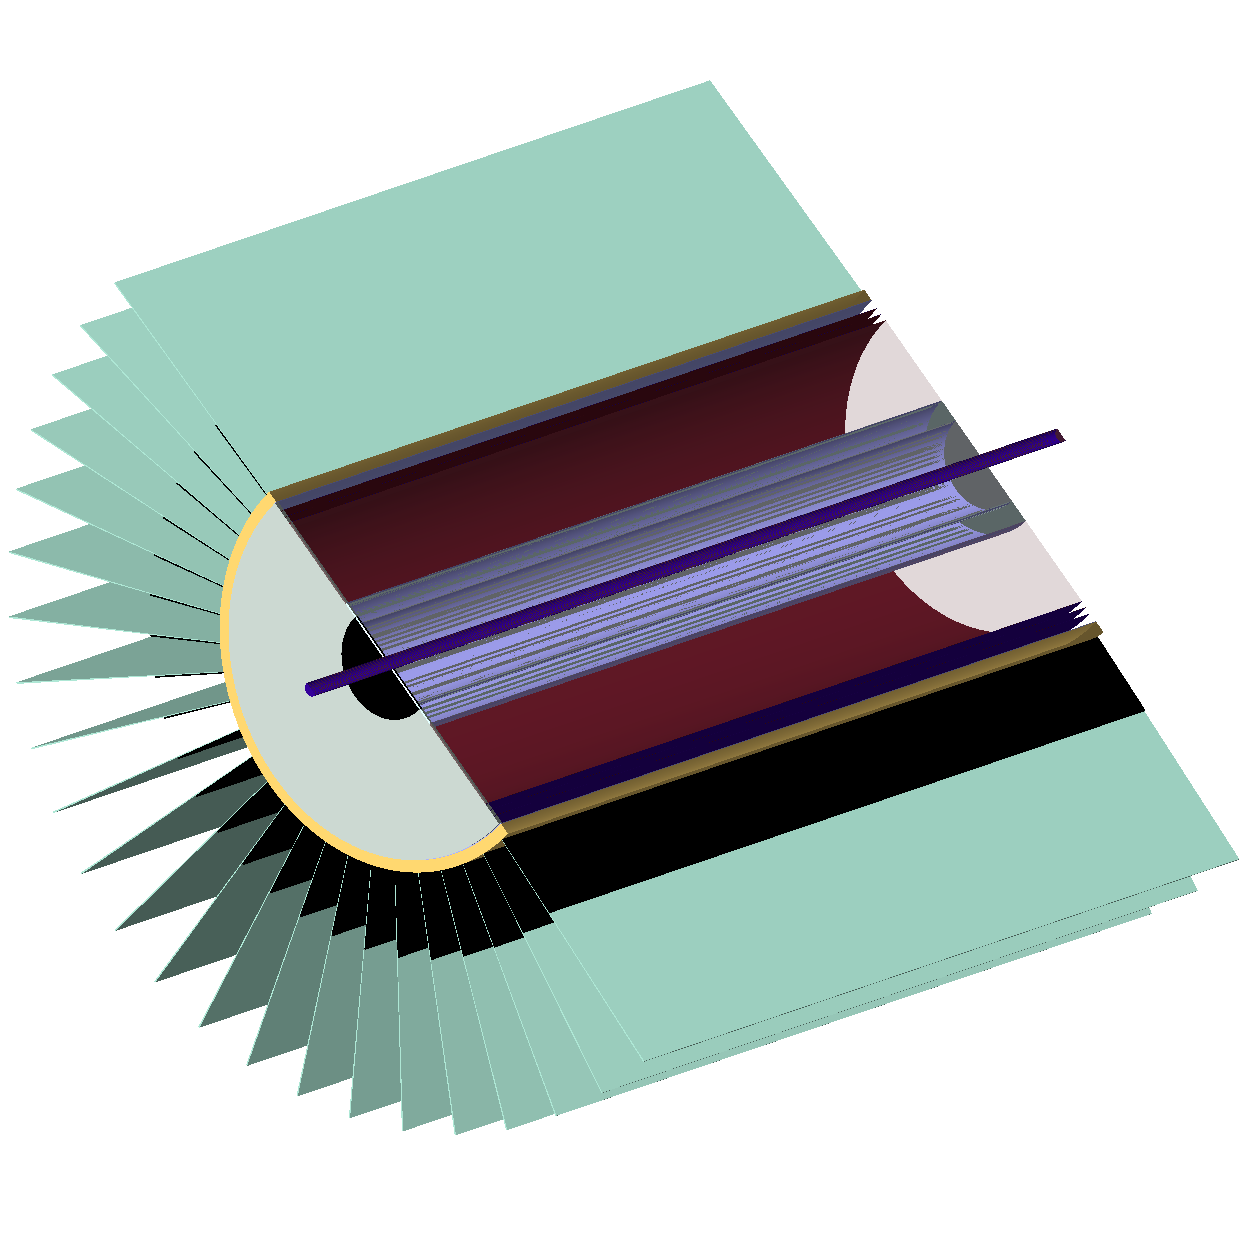
\includegraphics[width=0.8\linewidth]{figures/rtpc.png}
	\caption{BONuS12 RTPC geometry implemented in GEMC}
	\label{fig:gemc_rtpc}
\end{figure}
There are other variable names that you see within the detector attributes above that are important to understand. The variable \lstinline|style| describes whether the type is a solid (\lstinline|style| $= 1$) or wire frame (\lstinline|style| $= 0$). The \lstinline|sensitivity| variable directs GEMC to add the output of this region to the correct bank in the output file. In order to define what particle-interaction output variables appear in the output file for the given volume, we use the \lstinline|hit_type| variable. Hit type will be covered more in Section \ref{ss:drift_e} when we discuss what to do when ionization occurs in the drift region.

Not all of the RTPC details can be implemented into GEMC, so we only include the important components in the GEMC simulation. Those components include the main detector parts like the target, ground and cathode foils, GEM foils, and readout pad-board. Then there are the components that had to be included in order to understand their effect on the particles that may be traveling through them ($e.g.$ down-stream end plate, electronics and translation boards, support ribs and spines, etc). Most of these secondary components had to be simplified in order to save time during the simulation process. For example, a cylindrical volume of average density was included outside of the readout pad-board. This density included a proportional amount of the support ribs and spines, electronics, and air. The final geometry can be seen in Fig. \ref{fig:gemc_rtpc}, which shows half of the RTPC in order to see the internal structure. 

Once the geometry is set up for the RTPC, it must be inserted within the CLAS12 detectors in GEMC. The file that brings all these detectors together in GEMC is an XML ($i.e.$ extended markup language) file called a \textit{gcard}. This file is where one defines not only which detectors to include in the simulation, but also what variables to include in the output file and what the incoming particle beam should be ($e.g.$ momentum, angle, spread, etc.). For example, if one desired $10.6$ GeV/c electrons to travel at $0^{\circ}$ scattering angle $\theta$ and $0^{\circ}$ around $\phi$, with a spread of $\pm 10$ MeV/c in momentum, $\pm 10^{\circ}$ in $\theta$ and $\pm 180^{\circ}$ in $\phi$, the code would be:

\begin{lstlisting}
	<option name="BEAM_P"   value="e-, 10.6*GeV, 0.0*deg, 0.0*deg"/> 
	<option name="SPREAD_P" value="10*MeV, 10*deg, 180.0*deg"/>
	<option name="BEAM_V"   value="(0, 0, 0)cm"/>
	<option name="SPREAD_V" value="(0.3, 20)cm"/>
\end{lstlisting}
Notice that in this code snippet, the vertex of the particle \lstinline|BEAM_V| is set to zero and there is a spread on that vertex \lstinline|SPREAD_V| of $0$ cm $\leq r \leq 0.3$ cm and $-20.0$ cm $\leq z \leq 20$ cm), which spans the diameter and length of the BONuS12 RTPC target.

This method of generating particles makes use of GEMC's internal event generator. The particles that can be generated make use of the Geant4 particle bank. The trouble with this internal generator is that we don't have access to multiple particles that we may want to examine ($i.e.$ secondary particles). For that we have to look toward another method of generating particles and how to import that file into GEMC.

\subsection{Event Generator}
For the purpose of our GEMC simulations in BONuS12, we are primarily concerned with the reaction $eD \rightarrow e'pX$ and so we need a means of generating such events. For that we use an external particle generator called Pythia. Pythia is a program for generating high-energy physics events, which is precisely what we need. It uses theory and models on collisions between particles like $e^-$, $e^+$, $p$ and $\bar{p}$ ($i.e.$ anti-proton) to generate output in a file format name Lund, after the University where the program was developed.

\begin{table}[h!]
	\begin{center}
		\caption{Lund file header}
		\label{tab:lund_header}
		\begin{tabular}{r|c} % <-- Alignments: 1st column left, 2nd middle and 3rd right, with vertical lines in between
			\rowcolor{cyan} \textbf{Column} & \textbf{Quantity} \\
			\hline
			1 & \textbf{Number of particles} \\
			\rowcolor{lightgray} 2 & Mass number of the target \\
			3 & Atomic number of the target \\
			\rowcolor{lightgray} 4 & Target polarization \\
			5 & \textbf{Beam Polarization} \\
			\rowcolor{lightgray} 6 & Beam particle type \\
			7 & Beam energy (GeV) \\
			\rowcolor{lightgray} 8 & Interacted nucleon ID (proton or neutron) \\
			9 & Process ID \\
			\rowcolor{lightgray} 10 & Event weight \\
			\hline
		\end{tabular}
	\end{center}
\end{table}

This Lund output file format has very specific variables that we can take advantage of in GEMC. The first line of this Lund file contains header information for the particles to follow from the collision simulation. This header contains 10 different columns, listed in Table \ref{tab:lund_header}. The items in bold are used by GEMC. Given the number of particles listed under column 1, there will be a list below the header with particle details for each (see Table \ref{tab:lund_particles}). That is, if there is a 5 listed under the first column in the header, then below the header will be 5 lines for each of the particles. For a simulation with multiple events, subsequent events appear after the last particle of the previous beginning again with the header line.

\begin{table}[h!]
	\begin{center}
		\caption{Lund particles}
		\label{tab:lund_particles}
		\begin{tabular}{r|c} % <-- Alignments: 1st column left, 2nd middle and 3rd right, with vertical lines in between
			\rowcolor{cyan} \textbf{Column} & \textbf{Quantity} \\
			\hline
			1 & \textbf{Index} \\
			\rowcolor{lightgray} 2 & Lifetime [nanoseconds] \\
			3 & \textbf{Type (1 is active)} \\
			\rowcolor{lightgray} 4 & \textbf{particle ID} \\
			5 & Index of the parent \\
			\rowcolor{lightgray} 6 & Index of the first daughter \\
			7 & \textbf{momentum x [GeV]} \\
			\rowcolor{lightgray} 8 & \textbf{momentum y [GeV]} \\
			9 & \textbf{momentum z [GeV]} \\
			\rowcolor{lightgray} 10 & Energy of the particle [GeV] \\
			11 & Mass of the particle [GeV] \\
			\rowcolor{lightgray} 12 & \textbf{vertex x [cm]} \\
			13 & \textbf{vertex y [cm]} \\
			\rowcolor{lightgray} 14 & \textbf{vertex z [cm]} \\
			\hline
		\end{tabular}
	\end{center}
\end{table}

For the BONuS12 experiment, the event generator created a Lund file with various electron-proton deep-inelastic collisions that we must run through GEMC. To do this, instead of utilizing the GEMC internal event generator, we include the following line of code
\begin{lstlisting}
	<option name="INPUT_GEN_FILE" value="LUND, even_gen.lund"/>
\end{lstlisting}
in the gcard that we use to give direction to GEMC. This file will serve to instruct GEMC how many particles are in each event and the type of particle, its momentum and its vertex. For our purposes in BONuS12, we have Lund files with primary electron-proton events that also have a number of additional protons that serve as background. The number of these background protons can vary, but the intent is always to best represent what we would expect to see. Once we run this file through GEMC with all the other variables defined that have been previously discussed, we need to take a look at what happens in the simulation when these protons travel through the RTPC.

\subsection{Drift Electrons} \label{ss:drift_e}
When protons travel through the sensitive region of the RTPC, they ionize the gas creating what are known as ionization electrons. Because of the electric field within that sensitive region, those ionization electrons drift toward the outer edge of the RTPC to the readout electronics. The other thing that happens to protons traveling through the RTPC is that they bend in a helical pattern because of the magnetic field. The ionization electrons that are created also bend, but in the opposite direction of the protons because they are oppositely charged.
  
By how much these charged particles bend when moving through the magnetic field created by the solenoid magnetic depends, in part, on the magnitude of that field throughout their path. Therefore, it is very important to get an accurate map ($ie.$ the magnitude and direction of the field at small steps in space around the magnet) of that magnetic field. This is important for both the generation of simulated data and the reconstruction of real data. For the simulated data, the field map will define the path of both protons and ionization electrons within GEMC. For the real data, it will play a role in the reconstruction of kinematics from events.

\begin{figure}[h!]
	\centering
	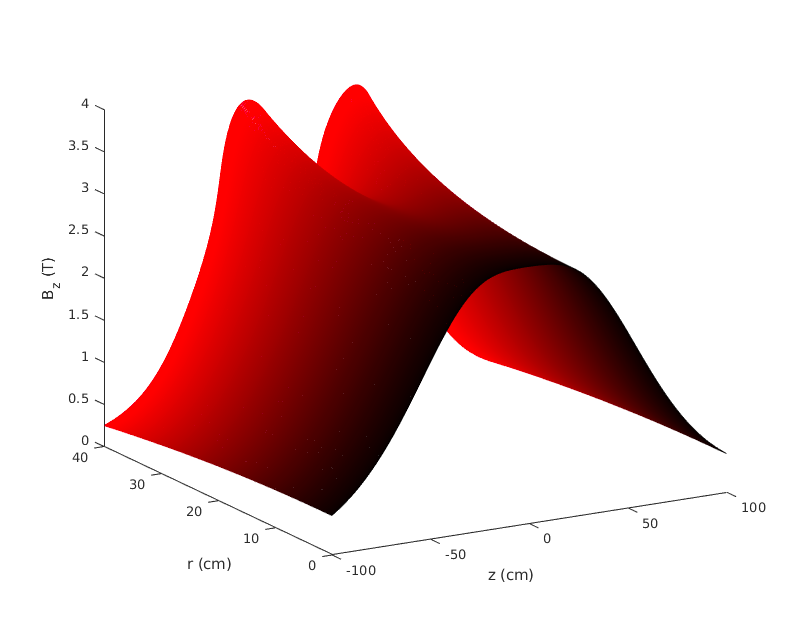
\includegraphics[width=0.8\linewidth]{figures/solenoid_map.png}
	\caption{CLAS12 Solenoid Field Map (V.Lagerquist)}
	\label{fig:clas12_solenoid_map}
\end{figure}

\begin{figure}[h!]
	\centering
	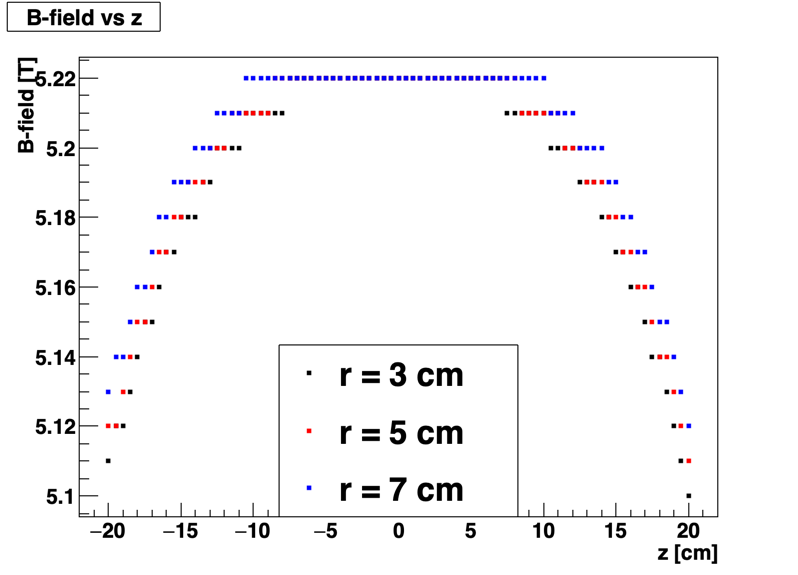
\includegraphics[width=0.8\linewidth]{figures/bfield.png}
	\caption{Magnetic field strength versus $z$ for values of $r$.}
	\label{fig:bfield}
\end{figure}

The field map for the solenoid magnet in CLAS12, in which the BONuS12 RTPC will reside, is mapped in steps of $z$ and $r$ (symmetric in $\phi$) by Victoria Lagerquist at Old Dominion University (see Fig. \ref{fig:clas12_solenoid_map}). Within the sensitive region of the RTPC ($i.e.$ $3$ cm $\leq r \leq 7$ cm),  the map looks like Fig. \ref{bfield} in steps of $z$ within the RTPC. The map itself takes as input course measurements of the B-field inside the solenoid and finds a more finely-structured field to use in other applications. One of those applications is the simulation of protons traveling through the RTPC. 

While GEMC does an acceptable job simulating the proton tracks, Garfield++ has a more specialized capacity to simulate the ionization electrons (also called drift electrons) created by the protons as they interact with the gas mixture as well as the electric and magnetic fields that are present in the sensitive region of the RTPC. The available build of Garfield++ does not allow for a magnetic field map to be imported, so it had to be written in as a custom feature. 

By starting electrons at different values of $r$ throughout the sensitive region ($i.e.$ 3 cm $\leq r \leq$ 7 cm) and using known values of the electric and magnetic fields, Garfield++ calculated the time it takes that electron to reach the outer edge of the RTPC ($i.e.$ 8 cm) as well as the change of angle that it makes. By defining more than one electron for Garfield++ to simulate, we can fit the results to a Gaussian to find the mean and sigma. Those means serve as points in the figures to follow of drift time and drift angle and the sigmas define the diffusion that occurs. As we will see in the coming sections, these drift times and drift angles are of crucial importance to the BONuS12 experiment. 

\subsection{Gas Optimization}
One of the first uses for the drift time and drift angle from Garfield++ is to optimize the gas mixture that will be used in the sensitive region of the RTPC. We want a fast drift time to ensure our electronics are able to handle the signal. This would also be less demanding on the trigger and usually means less diffusion. The other property to minimize, drift angle, would ensure that our track is discernible from others in the detector at the same time. Along this line is the need to minimize the diffusion in that occurs within the RTPC in order to increase the resolution of the hits. Thus, we need a gas mixture is that is fast, with small drift angle and diffusion properties, but with a high number of primary ionization events to reconstruct the track.

\begin{figure}[h!]
	\centering
	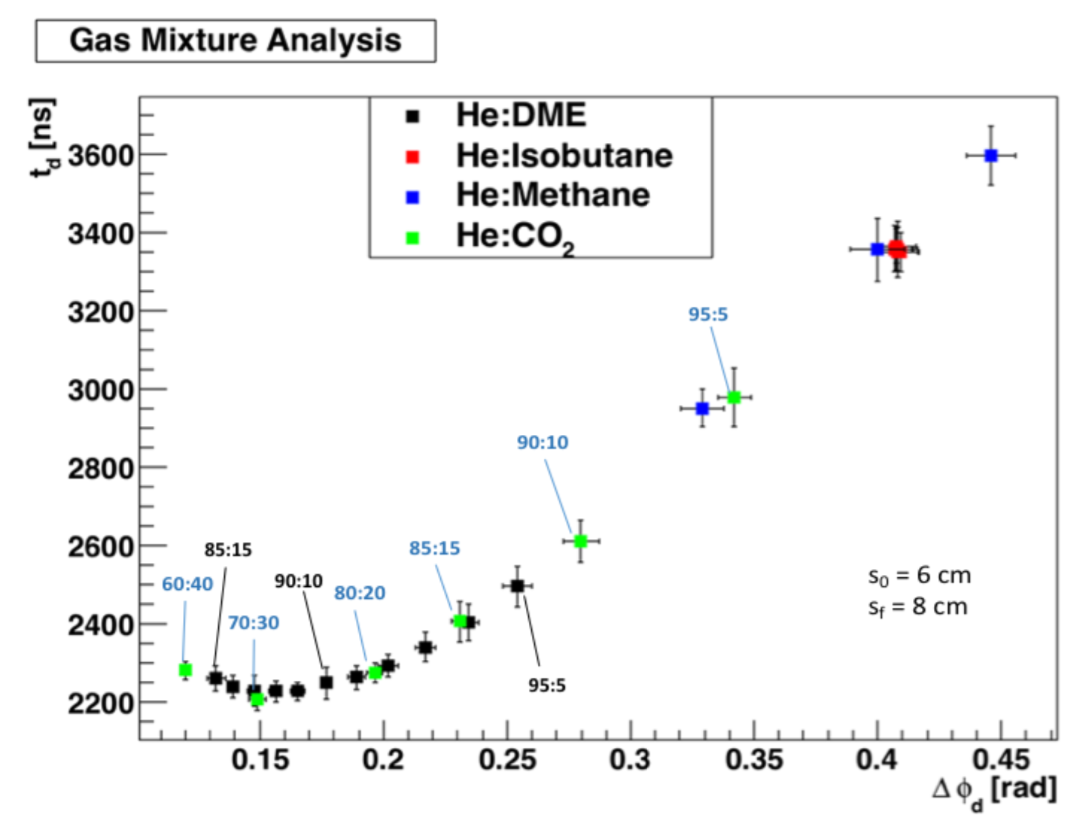
\includegraphics[width=0.8\linewidth]{figures/gas_opt_phi_vs_t.png}
	\caption{Drift angle vs drift time for various gas mixtures}
	\label{fig:gas_opt_phi_vs_t}
\end{figure}

The purpose of mixing gases is two-fold. First, there must be a primary gas where primary ionization occurs. Typically this is chosen to be a noble gas such as helium, neon, and argon A noble gas is usually the primary gas because the outer electron level of the molecule is full, meaning the gas would not interact with the walls of the detector. Also because the outer level is full, the probability of capturing a drift electron is low (i.e. they have a low electron affinity). Second, in order to prevent secondary effects such as photon feedback\footnote{Secondary avalanches created from decay through photon emission of excited primary gas atoms.} and field emission \footnote{Electrons emitted from an electric field.}, there must exist another gas to act as a quencher. This quencher gas is used to create a stable gas mixture that creates a signal well separated from noise of the electronics.

The first goal is to identify the type of quencher. Fig. \ref{fig:gas_opt_phi_vs_t} shows the drift time as a function of the drift angle of four gas mixtures in a sensitive region containing an electric field of 625 V/cm starting from 6 cm and ending at 8 cm. This electric field corresponds to a potential of -2500 V within the sensitive region, which is high enough to move ionization electrons to the GEMs, but lower than the breakdown potential of the gas (more about this in a few paragraphs). These initial and final radii were chosen to gather results quickly. The error bars on these points are the sigmas of the Gaussian fits of the histogram and represent the diffusion properties of the mixture.

All ratios of He-Isobutane result in almost identical drift angle and drift time. The He-DME starts with a ratio of 85:15 on the far left of Fig. \ref{fig:gas_opt_phi_vs_t} and goes to 100:0 on the far right. The mixture of 87:13 He:DME is at the minimum of the curve. Ideally, as in the original BONuS6 experiment, we could chose this He-DME mixture. However, in an effort to chose a non-flammable gas, we decided to take a look at He-CO$_2$ mixtures.

\begin{figure}[h!]
	\centering
	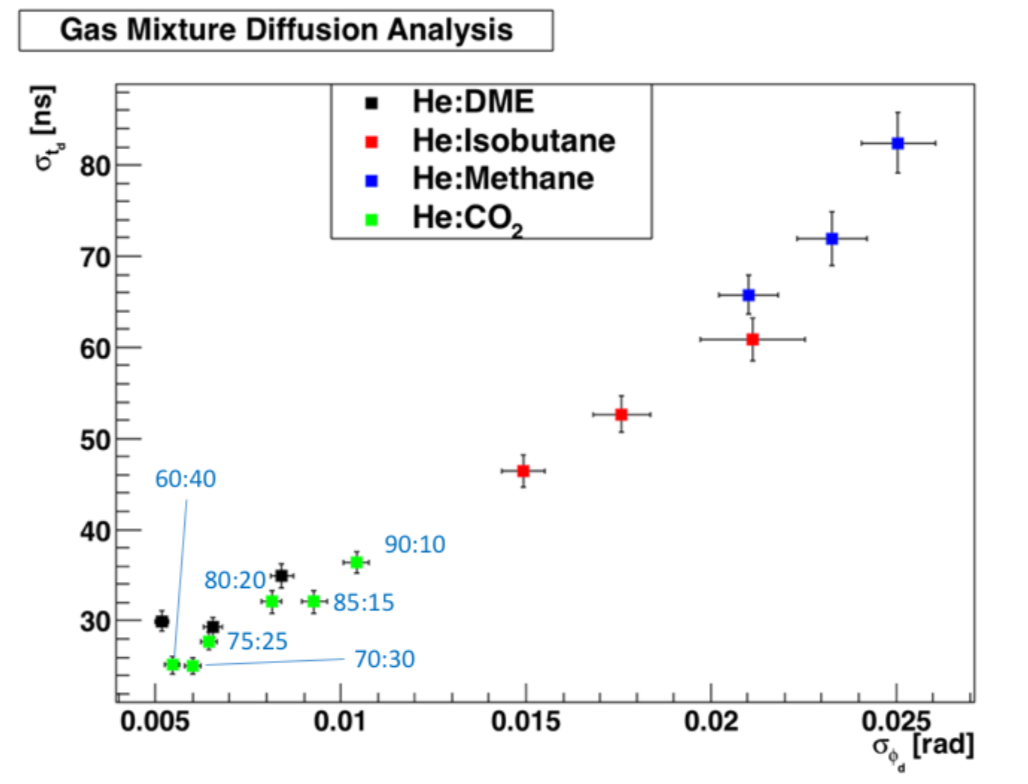
\includegraphics[width=0.8\linewidth]{figures/gas_opt_sigphi_vs_sigt.png}
	\caption{Diffusion in drift angle vs diffusion in drift time for various gas mixtures}
	\label{fig:gas_opt_sigphi_vs_sigt}
\end{figure}

In Fig. \ref{fig:gas_opt_phi_vs_t}, the He-CO$_2$ mixture is in green with the ratios labeled in blue. The 70:30 mixture is at the minimum drift time,which certainly meets the criteria for BONuS12. One of the characteristics that we need to identify during a run is when there may be slight changes in the gas mixture. If we chose to be at the minimum, then identifying when a change occurs would be difficult. This is because while there may be a change in drift angle as the ratio changes, at the minimum there the drift time changes are on the order of nanoseconds. If 80:20 is chosen, then we could more easily identify if a change happens during a run by the noticeable change in both drift angle and drift time. For this reason as well as its non-flammability, the best choice of a gas mixture would be 80$\%$:20$\%$ He:CO$_2$.

\begin{figure}[h!]
	\centering
	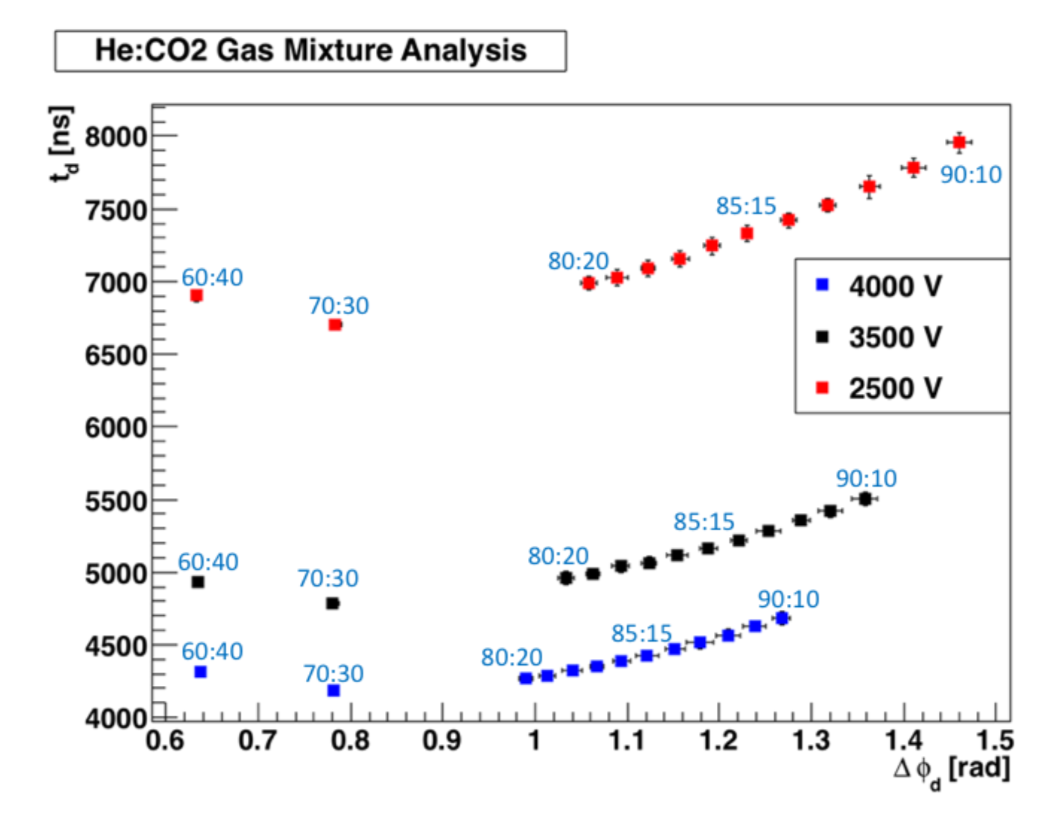
\includegraphics[width=0.8\linewidth]{figures/gas_opt_pot.png}
	\caption{Drift time versus drift angle for He:CO$_2$ using various potentials.}
	\label{fig:gas_opt_pot}
\end{figure}

Now we must look at reducing diffusion effects for this mixture or at least understand what those effects are for our chosen mixture and potential. If we look at a plot of the diffusion in $\phi$ ($i.e. \sigma_{\phi_{d}}$) as a function of diffusion in time ($\sigma_{t_{d}}$) as in Fig.
\ref{fig:gas_opt_sigphi_vs_sigt}, we see that the mixtures of He-CO$_2$ rival those of He-DME for ratios of 80:20-75:25. Given this plot alone, it can be concluded that mixtures below 75:25 of He-CO$_2$ do better than the He:DME mixtures.

The next step in this optimization is to look at the potential within the sensitive region of the RTPC. Here, note that preliminary experimental studies showed that the maximum voltage on the cathode would be about -4000 V for He-CO$_2$. These studies were done with a flat prototype, so if we include that the cathode will be cylindrical, the potential may need to be less. Fig. \ref{fig:gas_opt_pot} is a plot of He-CO$_2$ mixtures for potentials of -2500 V, -3500 V, and -4000 V. Again, the error bars represent the diffusion properties of the mixtures, which comes from the sigma of the Gaussian fit to the histogram. As one would expect, the higher potential, the faster the drift time and the smaller the drift angle.

Given all of this information and the requirements of the detector, we chose a gas mixture of helium-carbon dioxide with a ratio of 80:20 at -3500V. The mixture He-CO$_2$ meets the requirement of being fast with a small drift angle. For low momentum ions, such as protons in the case of the BONuS12 experiment, reducing multiple scattering is accomplished with low-mass gas mixtures. Thus He-CO$_2$ is ideal. The CO$_2$ in the mixture does not serve so much as a quencher, since helium essentially acts as its own quencher, but does limit the diffusion that occurs within the region. In addition, CO$_2$ is nonflammable.

\subsection{Drift Equations}
By knowing the drift time and drift angles of electrons starting at various values of $r$ and $z$, we can plot the points and fit the points to an equation. These fit equations can be seen in the plots of $t_d$ vs. $r$ and $\phi_d$ vs. $r$ ($i.e.$ Fig. \ref{fig:drifte_t_vs_r} and Fig. \ref{fig:drifte_phi_vs_r}, respectively). We can then use these equations in GEMC to find the drift time and drift angle of a drift electron created at any point along the path of the proton in the sensitive region of the RTPC. In order to speed up simulation efforts, simulation electrons were created at $r = 3$ cm to $r = 7$ cm at $0.5$ cm increments and $z = -19$ cm to $z = 19$ cm at $5$ cm increments. This give us 81 data points to work with ($i.e.$ 9 points per fit line).

\begin{figure}[h!]
	\centering
	\begin{subfigure}[b]{0.49\textwidth}
		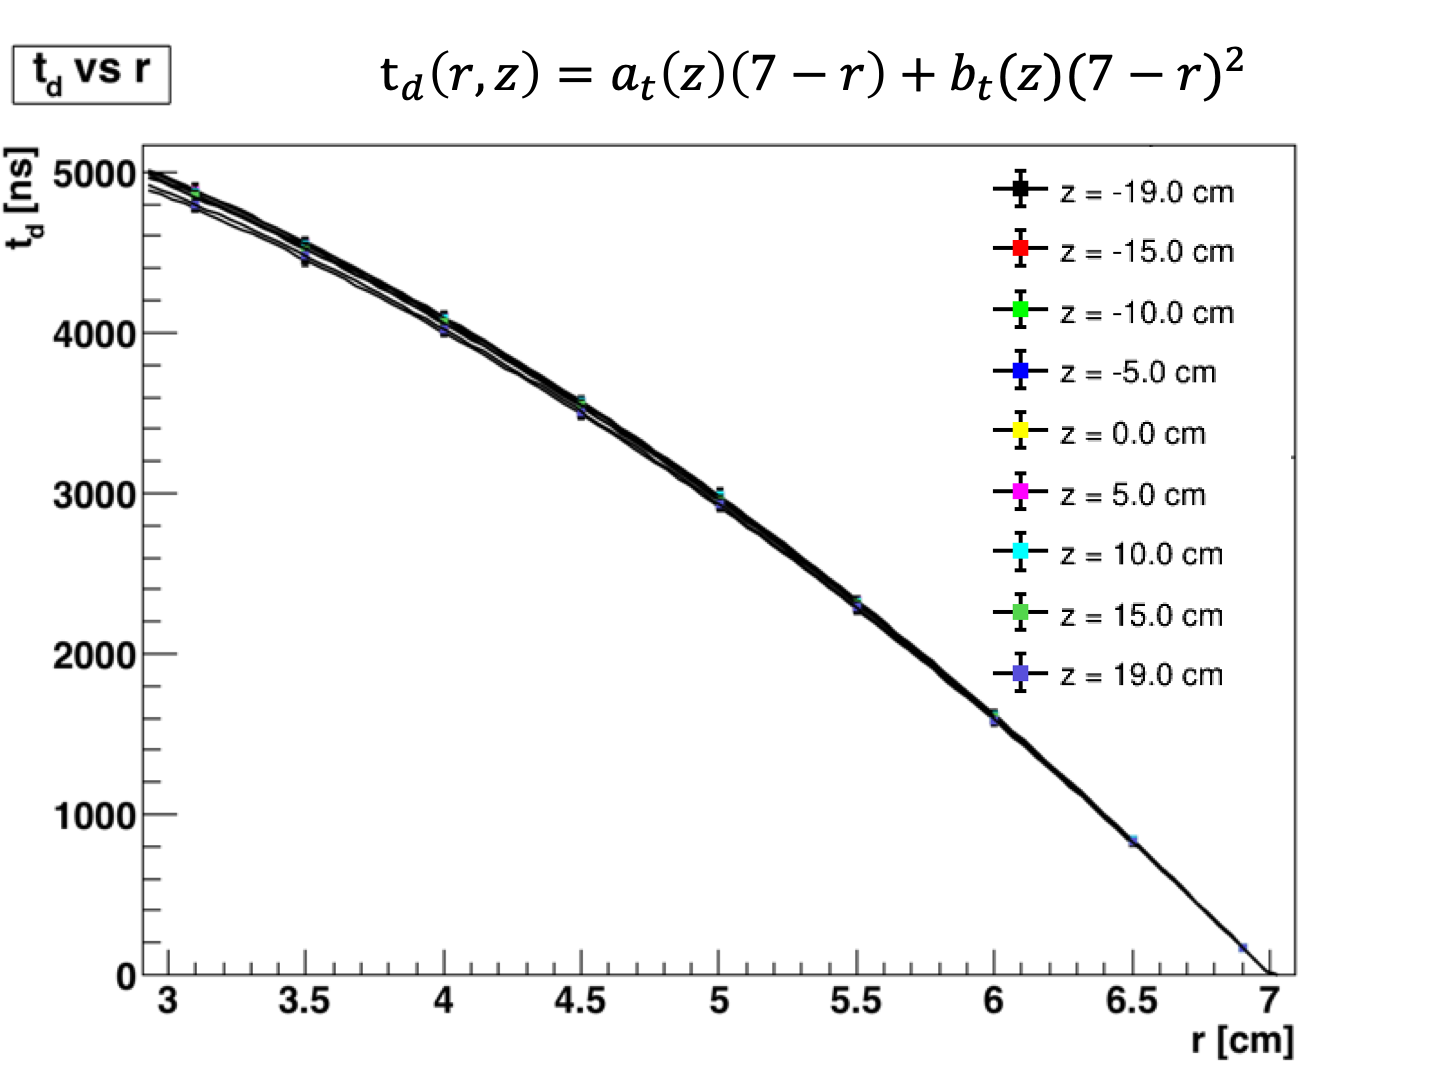
\includegraphics[width=\textwidth]{figures/drifte_t_vs_r.png}
		\caption{Drift time ($t_d$) vs. $r$.}
		\label{fig:drifte_t_vs_r}
	\end{subfigure}
	\begin{subfigure}[b]{0.49\textwidth}
		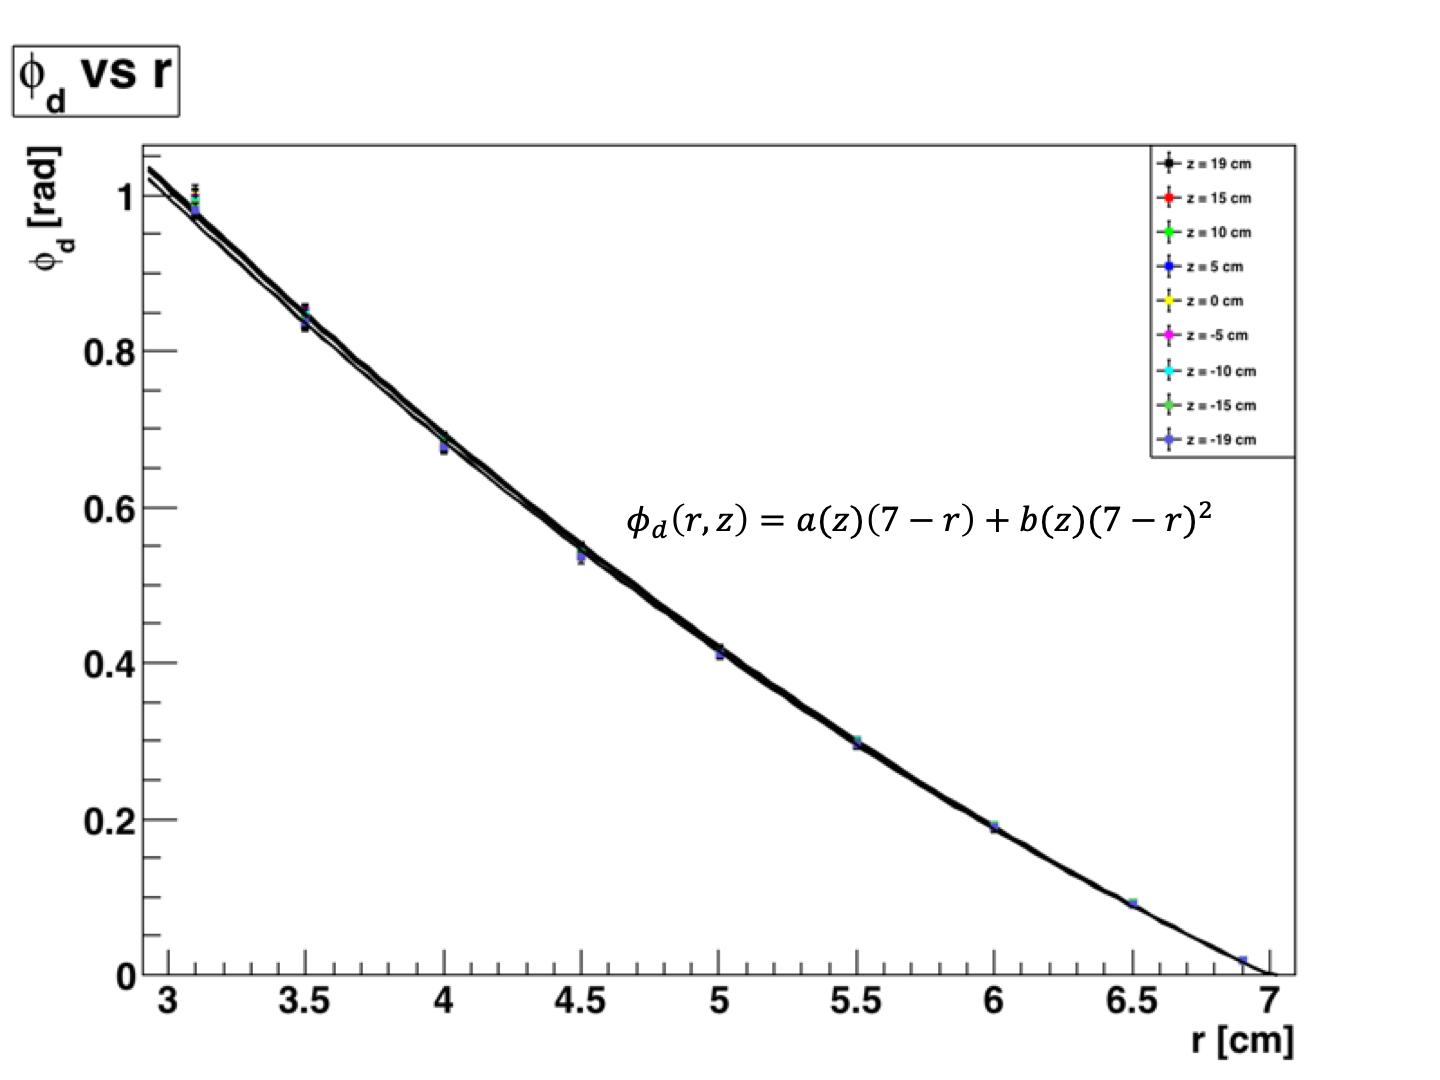
\includegraphics[width=\textwidth]{figures/drifte_phi_vs_r.png}
		\caption{Drift angle ($\phi_d$) vs. $r$.}
		\label{fig:drifte_phi_vs_r}
	\end{subfigure}
	\caption{Plots of drift electron properties.}
\end{figure}

The 9 points for each value of $z$ are fit to a second-order polynomial whose coefficients $a$ and $b$ depend on $z$. This is because the magnetic field changes with $z$, as shown in Fig. \ref{fig:bfield}, for three values of $r$ that are within the sensitive region of the RTPC. For each of the fit lines, or values of $z$, we extract the values of $a$ and $b$ for both drift time and drift angle. These values are shown in Fig. \ref{fig:drifte_a_and_b} and then fit to functions.

\begin{figure}[h!]
	\centering
	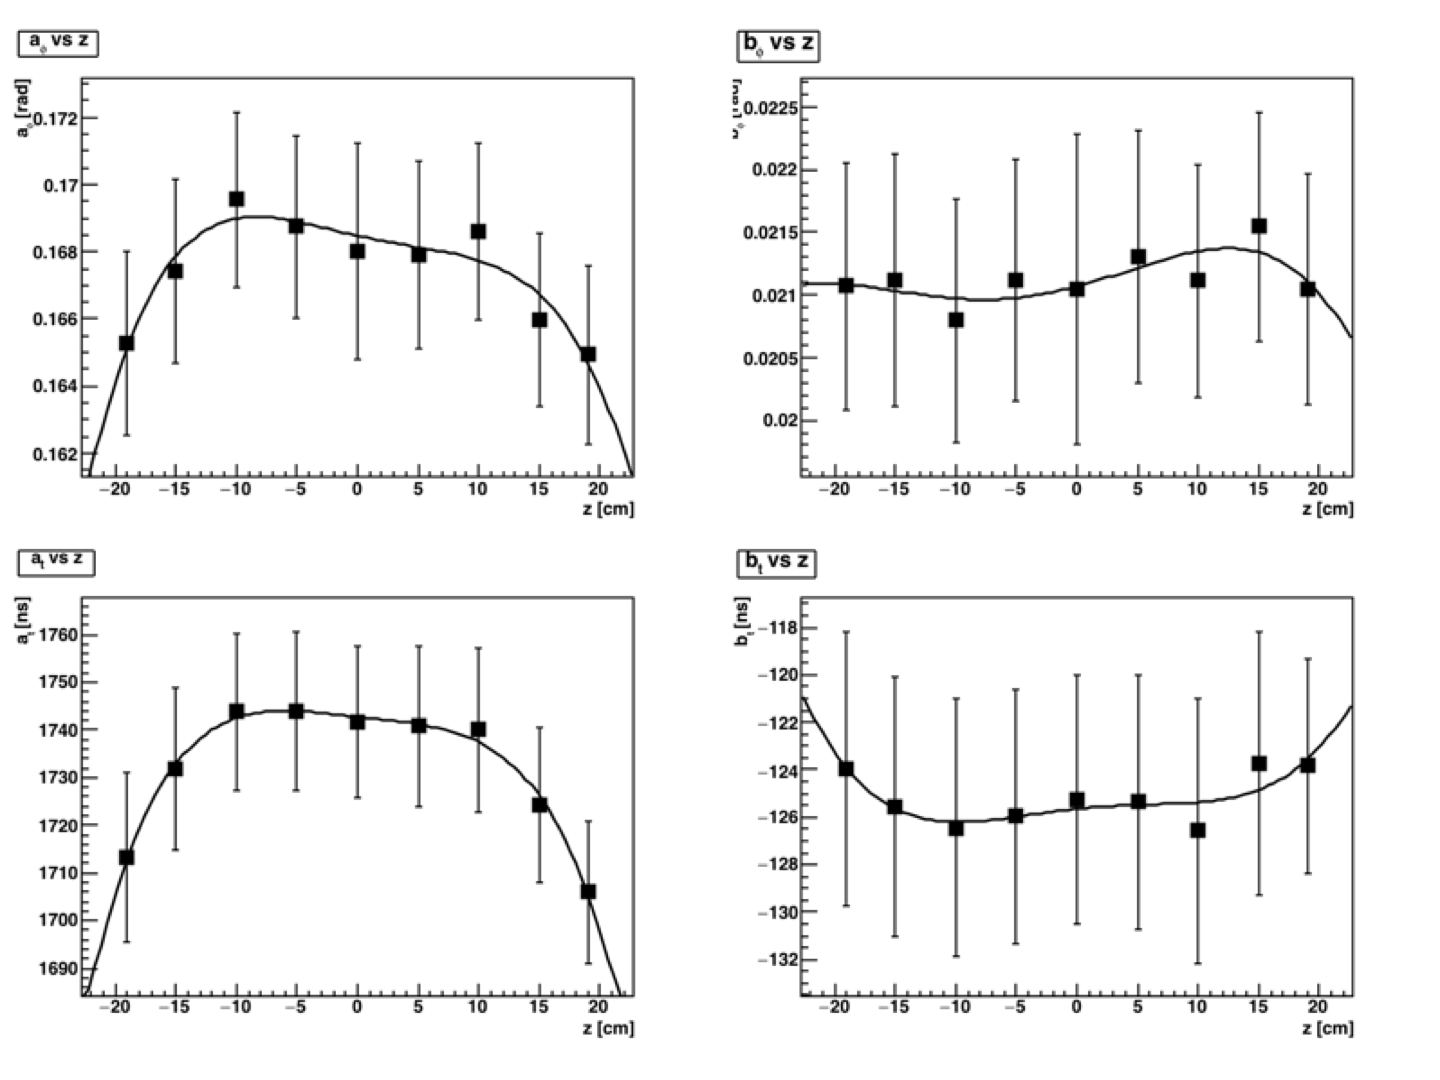
\includegraphics[width=0.8\linewidth]{figures/drifte_a_and_b.png}
	\caption{Parameters $a$ and $b$ for drift angle ($a_{\phi}$ and $b_{\phi}$) and drift time ($a_t$ and $b_t$).}
	\label{fig:drifte_a_and_b}
\end{figure}

The points in Fig. \ref{fig:drifte_a_and_b} plots are all fit to fourth-order polynomials because of the shape of the magnetic field (see Fig. \ref{fig:bfield}). These extracted functions defining the coefficients $a$ and $b$ for the drift time and drift angle are
\begin{eqnarray}\label{eqn:drifte_parameters}
\nonumber
a_{\phi}(z) &= a_{\phi0}z^4 +  a_{\phi1}z^3 +  a_{\phi2}z^2 +  a_{\phi3}z +  a_{\phi4} \\
\nonumber
b_{\phi}(z) &= b_{\phi0}z^4 +  b_{\phi1}z^3 +  b_{\phi2}z^2 +  b_{\phi3}z +  b_{\phi4} \\
\nonumber
a_t(z) &= a_{t0}z^4 +  a_{t1}z^3 +  a_{t2}z^2 +  a_{t3}z +  a_{t4} \\
b_t(z) &= b_{t0}z^4 +  b_{t1}z^3 +  b_{t2}z^2 +  b_{t3}z +  b_{t4}.
\end{eqnarray}
These equations go into the \lstinline|rtpc_hitprocess| class of GEMC. Therefore, when an ionization occurs in the simulation, GEMC uses those equations in Fig. \ref{fig:drifte_phi_vs_r} and Fig. \ref{fig:drifte_t_vs_r} to calculate the position of the ionization electron when it reaches the outer edge of the RTPC.

\section{DMS Simulations}
As we have seen in the previous sections, the drift of the ionization electrons is very sensitive to the gas mixture, temperature, pressure and potential. The Drift-Gas Monitoring System (DMS) had to be designed to measure any fluctuations in those parameters of the gas by way of measuring drift velocity (see Section \ref{sec:dms}). In order to do that, simulations of the DMS had to be done to optimize the uniformity of the electric field within the drift region as well as the geometry of the chamber itself.
\subsection{Geometry}
The parameters of interest to investigate and optimize were the anode diameter, diameter of the electrodes, and the distances between components. In order to look at these parameters, the geometry of the DMS was implemented into Garfield++, which consisted of its rectangular frame, grounded anode enclosure, anode wire, cathode plate, and field-shaping electrodes. 

The first step is to define the gas mixture and geometry of the box used to house all of the DMS components. By using the  \lstinline|Sensor| class in Garfield++, the framework and wires necessary to see the DMS response was built. Then, as seen in the code snippet below, grounded planes were placed along the box. 
\label{code:g++geodef}
\begin{lstlisting} 
// Setup the gas
MediumMagboltz* gas = new MediumMagboltz();
gas->SetComposition("He",80.,"CO2",20.);
gas->SetTemperature(293.);
gas->SetPressure(760.);
gas->EnableDrift();             // Allow for drifting in this medium
gas->PrintGas();

// Build the geometry
GeometrySimple* geo = new GeometrySimple();
SolidBox* box = new SolidBox(L_x/2., L_y/2., L_z/2., L_x/2., L_y/2., L_z/2.);
geo->AddSolid(box, gas);

// Make a component with analytic electric field
ComponentAnalyticField* comp = new ComponentAnalyticField();
comp->SetGeometry(geo);

// Create a sensor for readouts
Sensor* sensor = new Sensor();
sensor->AddComponent(comp);

// Create grounded planes at the edges of the box
comp->AddPlaneX(0.,0.,"x_min");
comp->AddPlaneX(L_x,0.,"x_max");
comp->AddPlaneY(0.,0.,"y_min");
comp->AddPlaneY(L_y,0.,"y_max");

comp->AddReadout("x_min");
comp->AddReadout("x_max");
comp->AddReadout("y_min");
comp->AddReadout("y_max");

sensor->AddElectrode(comp, "x_min");
sensor->AddElectrode(comp, "x_max");
sensor->AddElectrode(comp, "y_min");
sensor->AddElectrode(comp, "y_max");
\end{lstlisting}
Next, the anode and ground plate surrounding that wire was defined. The following code snippet shows the anode wire defined by a single declaration.
\begin{lstlisting} 
// Anode
comp->AddWire(x_0 + r_a + wall_d/2., L_y/2, dAnode, vAnode, "a", 100., 50., 19.3);
comp->AddReadout("a");
sensor->AddElectrode(comp, "a");
\end{lstlisting}
The ground plate surrounding the anode was constructed from a number of large-diameter grounded wires that were placed to form that shape of that plate, since Garfield++ has a difficulties with these rather complicated structures. The same was done for the cathode plate, which used two layers of wire components. The electrode wires were all placed individually, with one example in the code snippet below.
\begin{lstlisting}
comp->AddWire(dist, L_y/2.+b/2.+(i*s_y), dWire, Ex*(s_1 + (j*s_x)), name, 100., 50., 19.3);
comp->AddReadout(name);
sensor->AddElectrode(comp, name);
\end{lstlisting}
The function \lstinline|AddWire(double x, double y, double D, double V, string label, double L, double T, double rho)|, places the wire at \lstinline|x| and \lstinline|y| with diameter \lstinline|D|, potential \lstinline|V|, label of the wire, length \lstinline|L|, tension \lstinline|T|, and density \lstinline|rho| in that order. This placement was repeated 60 times completing 10 rows of electrodes with 6 wires comprising each electrode.

\subsection{Electric Field}
Once the geometries and code were in place, simulations to optimize those geometries were done to optimize the electric field. The primary concern was ensuring near-homogeneity of the electric field within the sensitive region. In order to look at that electric field, we need to look at the field profile along the plane where the anode lies. 

Fig. \ref{fig:e_map} shows the contour map of the field, whose surface contour quantities are on the right legend. The plot in Fig. \ref{fig:e_map} is made using the \lstinline|FieldView()| class. The potential from the cathode through to the electrodes was set to mirror what the electric field would be inside the RTPC ($i.e.$ 875 V/cm). The profile of the field along the line at $y=3$ cm is shown in Fig. \ref{fig:eprof_good} and Fig. \ref{fig:eprof_goodzoom} shows a zoom in to between the two sources to ensure its homogeneity ($i.e.$ a straight line). These plots are created using the \lstinline|PlotProfile()| function of the \lstinline|FieldView()| class.

\begin{figure}[h!]
	\centering
	\begin{subfigure}[b]{0.33\textwidth}
		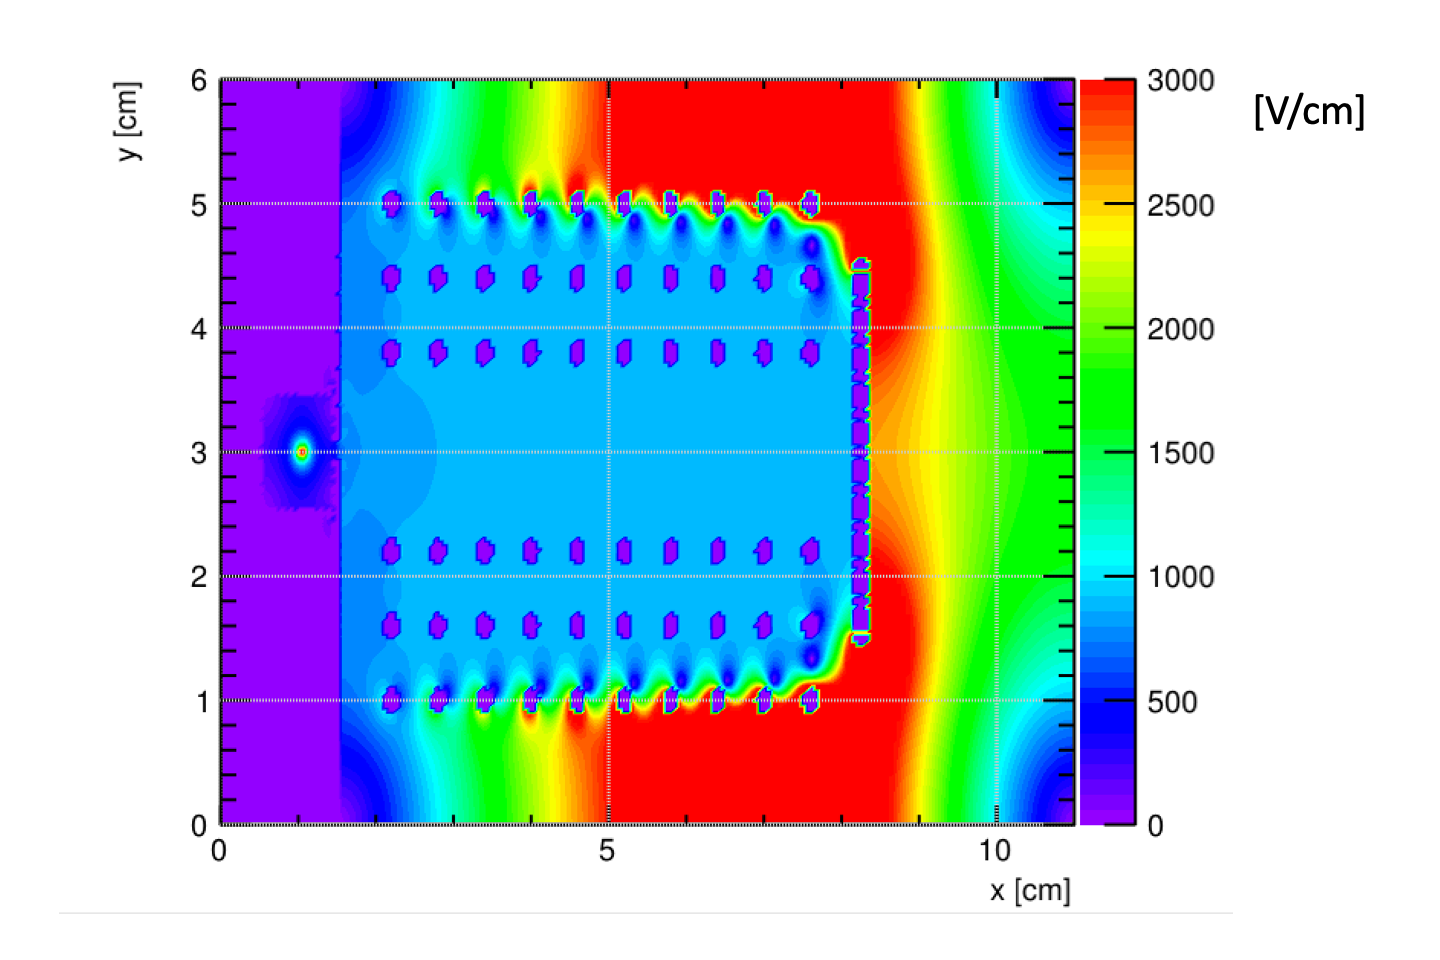
\includegraphics[width=\textwidth]{efield.png}
		\caption{Electric-field contour map along the cross-section in $x-y$ plane.}
		\label{fig:e_map}
	\end{subfigure}
	\begin{subfigure}[b]{0.3\textwidth}
		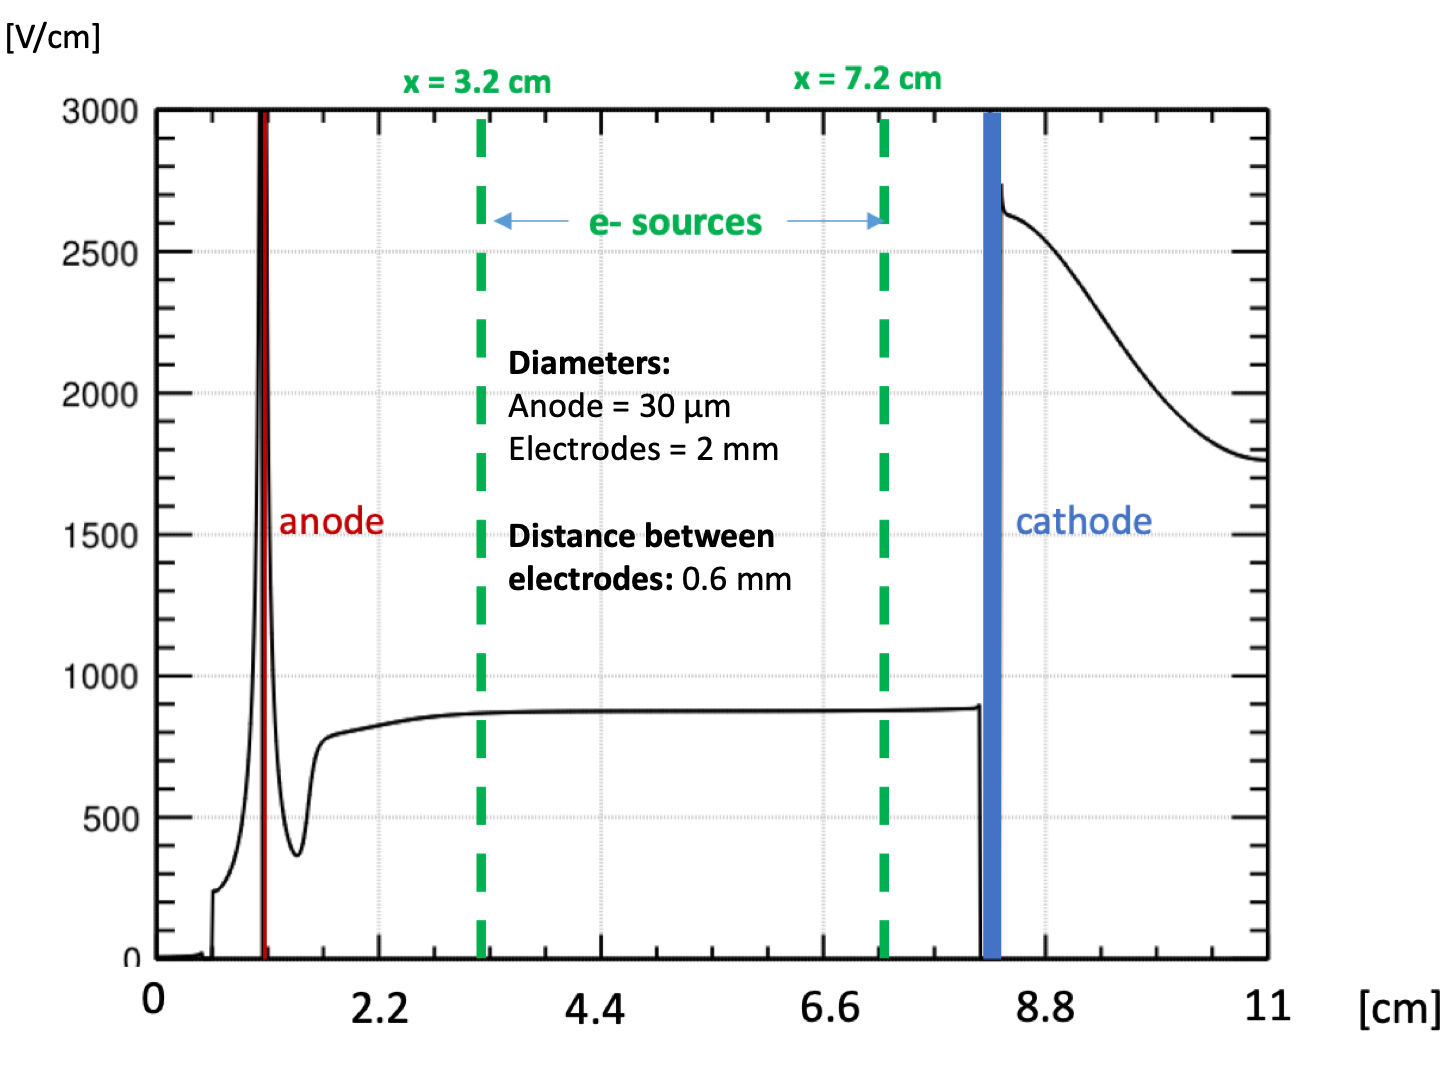
\includegraphics[width=\textwidth]{efield_goodsep.png}
		\caption{Electric-field profile along the plane of the anode.}
		\label{fig:eprof_good}
	\end{subfigure}
	\begin{subfigure}[b]{0.33\textwidth}
		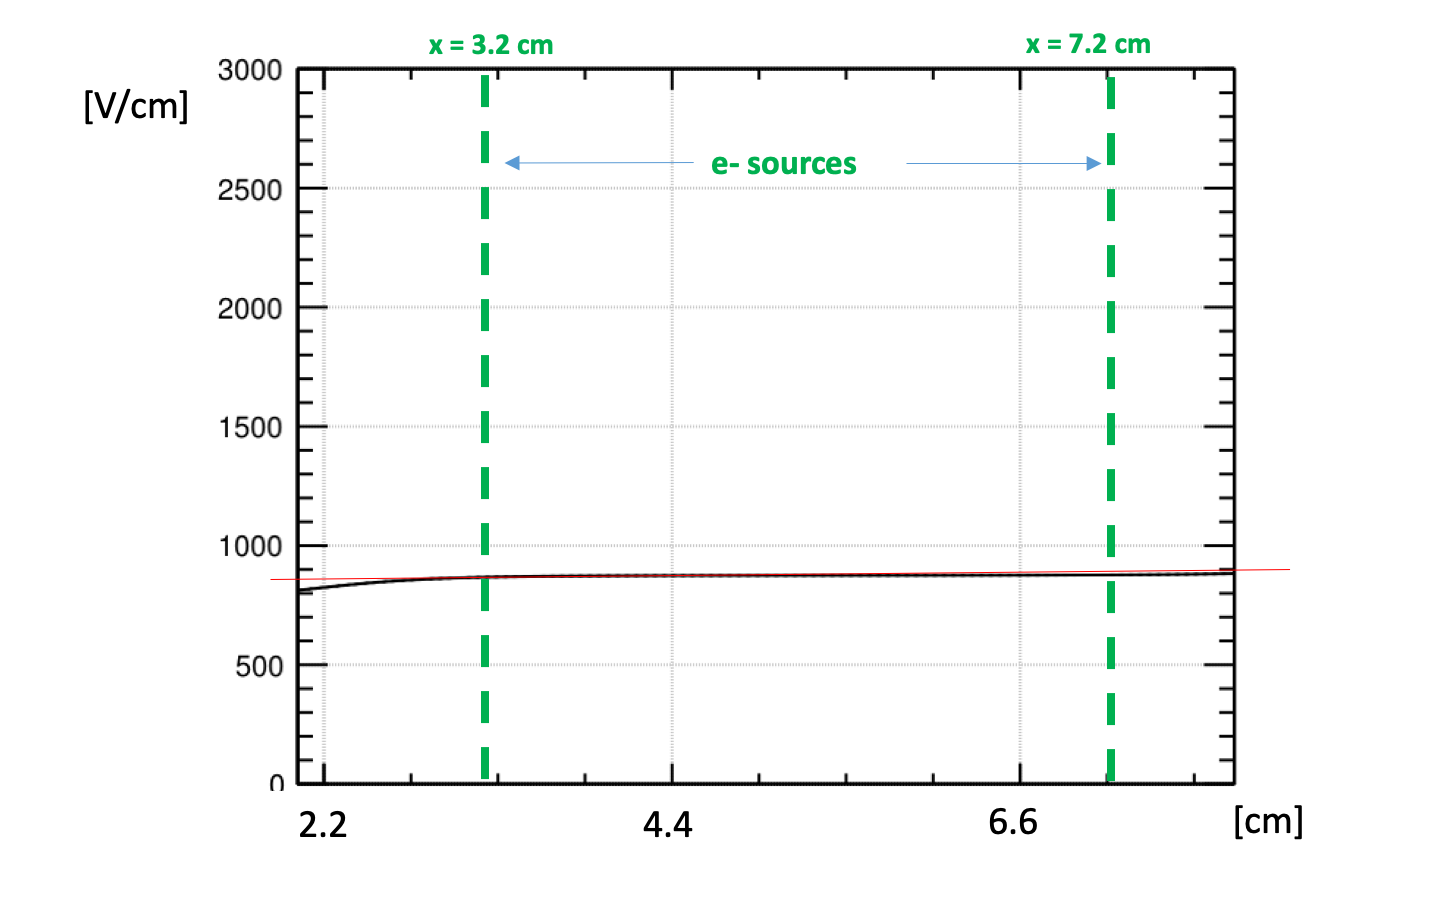
\includegraphics[width=\textwidth]{efield_zoom.png}
		\caption{Zoomed in electric-field profile to between the two sources.}
		\label{fig:eprof_goodzoom}
	\end{subfigure}
	\caption{Simulations of electric field within the DMS. In the profile plots in (b) and (c), the cathode and anode's locations are denoted as blue and red lines respectively. The sources and PMT's location and subsequent electron beams are pictured as green dotted lines.}
\end{figure}

To achieve this straight line indicative of homogeneity, many simulations took place varying the electrode diameter and distance. The progression of these simulations can be seen in Fig. \ref{fig:eprof}, beginning with small diameter electrodes ($i.e.$ 50 \textmu m) and a distance of 1.2 mm between each electrode (see Fig. \ref{fig:eprof_bigsep}). The small diameter coupled with the rather large distance between electrodes creates the large waves of field, which is not at all homogeneous. Fig. \ref{fig:eprof_midsep} shows the field profile with thicker electrodes ($i.e.$ 1 mm), but the same separation as Fig. \ref{fig:eprof_bigsep} ($i.e.$ 1.2 mm). The waves of the field seem to be calmer, but still inhomogeneous.

\begin{figure}[h!]
	\centering
	\begin{subfigure}[b]{0.30\textwidth}
		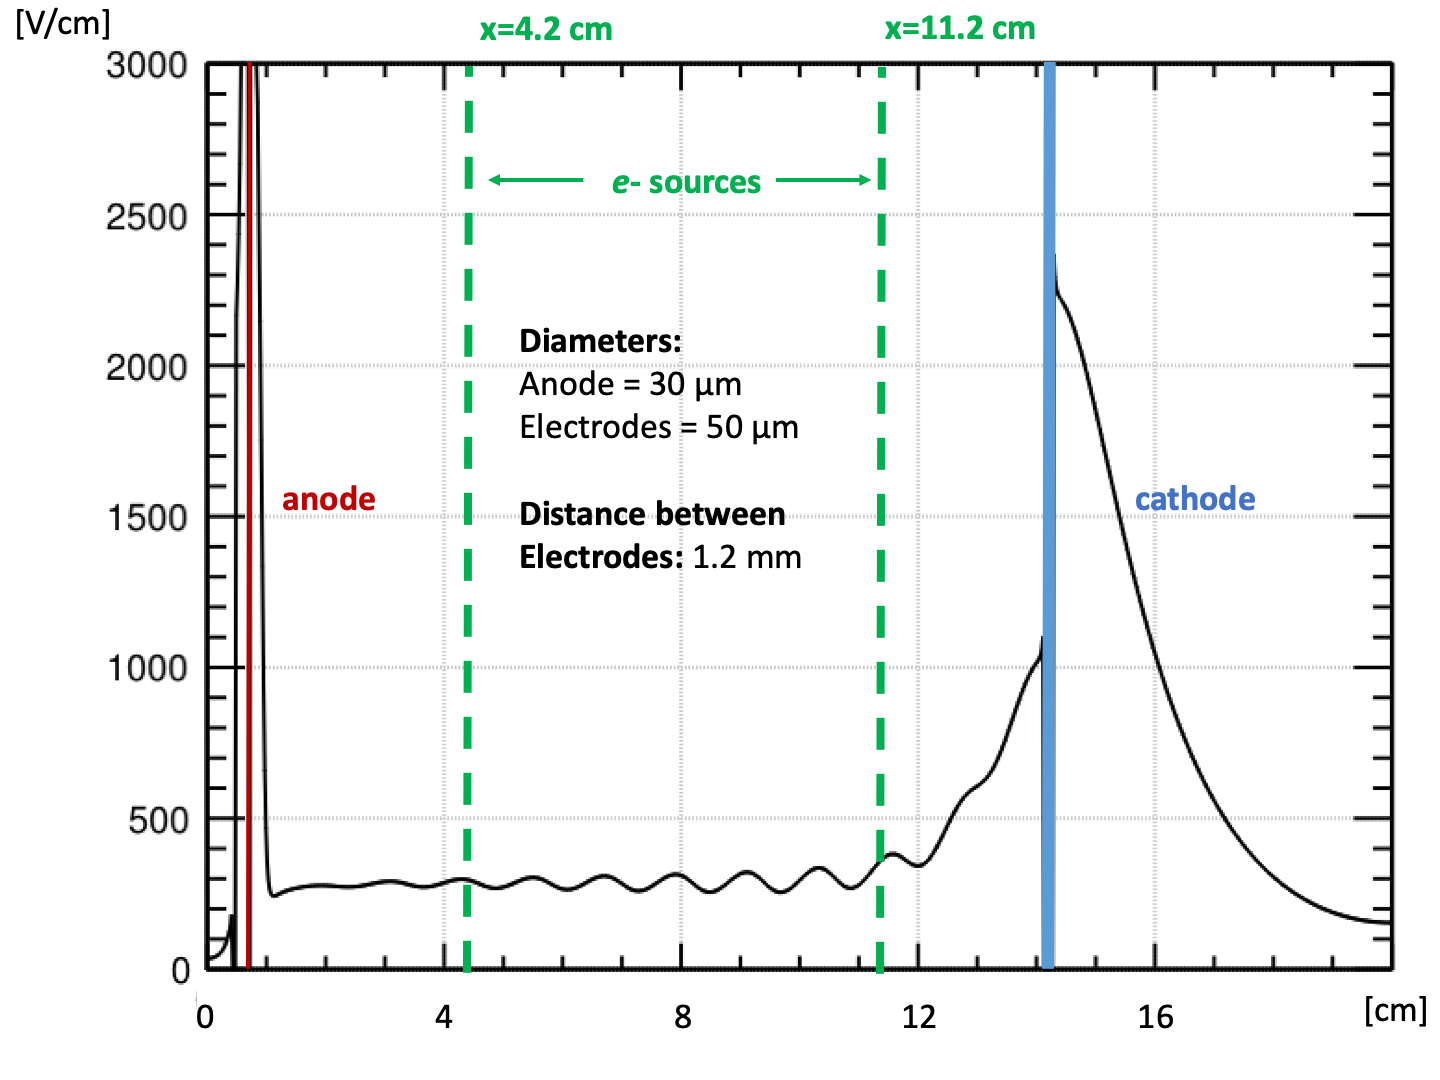
\includegraphics[width=\textwidth]{efield_bigsep.png}
		\caption{Electric field profile with electrode separation of 1.2 mm and diameter of 50 \textmu m.}
		\label{fig:eprof_bigsep}
	\end{subfigure}
	\begin{subfigure}[b]{0.30\textwidth}
		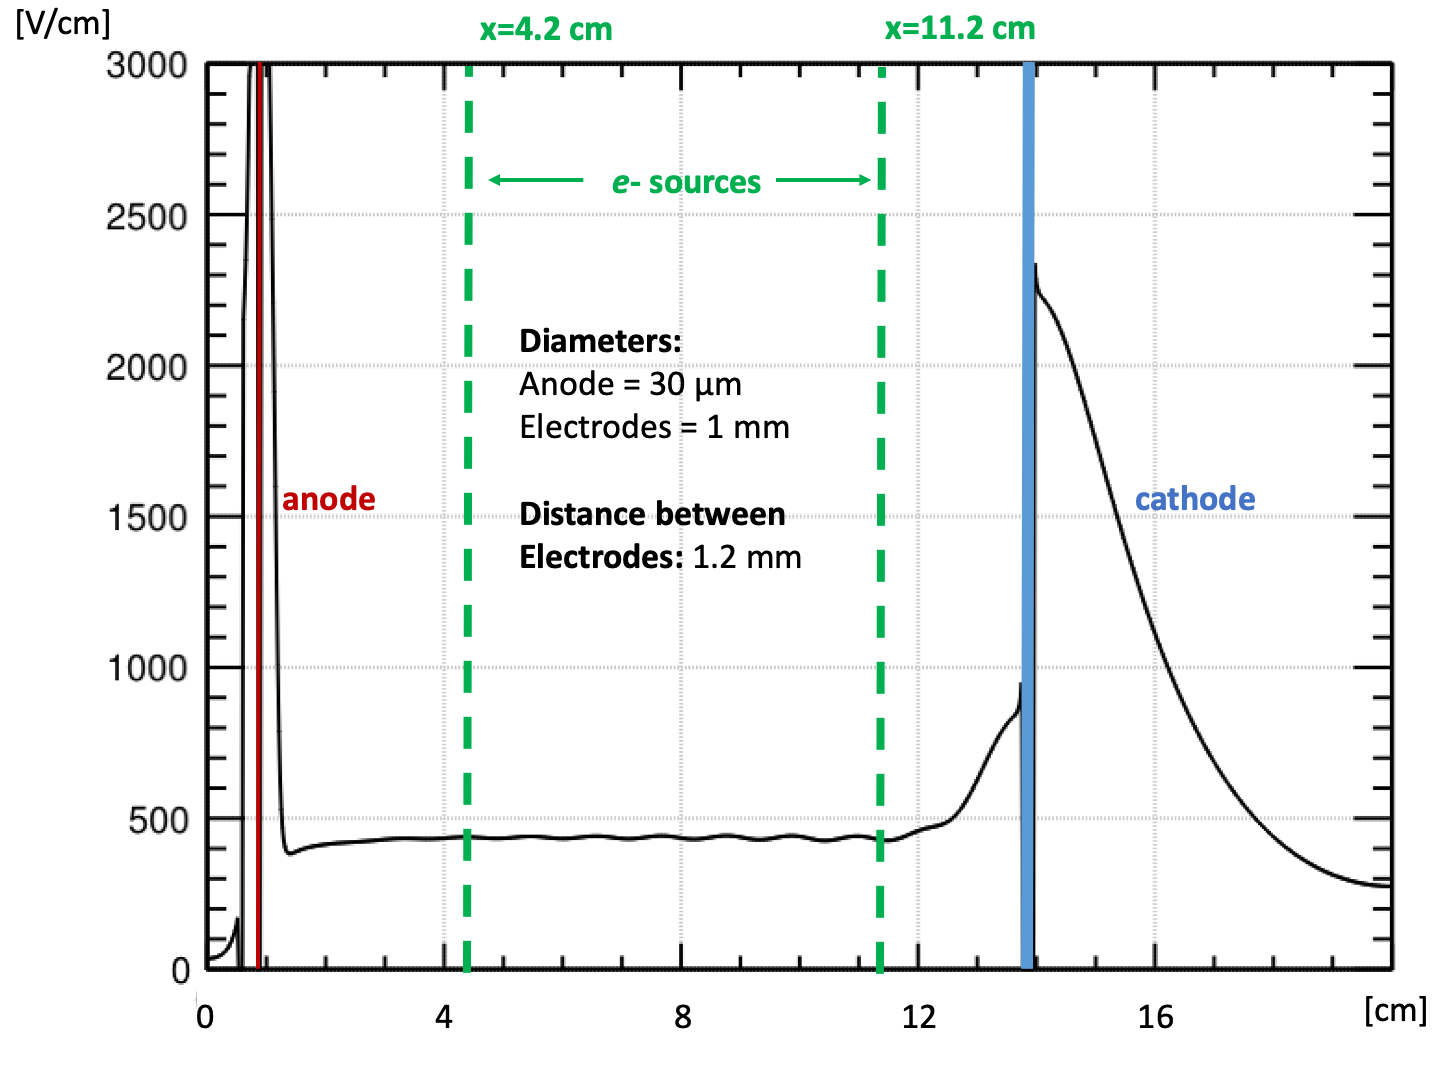
\includegraphics[width=\textwidth]{efield_midsep.png}
		\caption{Electric field profile with electrode separation of 1.2 mm and diameter of 1 mm.}
		\label{fig:eprof_midsep}
	\end{subfigure}
	\begin{subfigure}[b]{0.30\textwidth}
		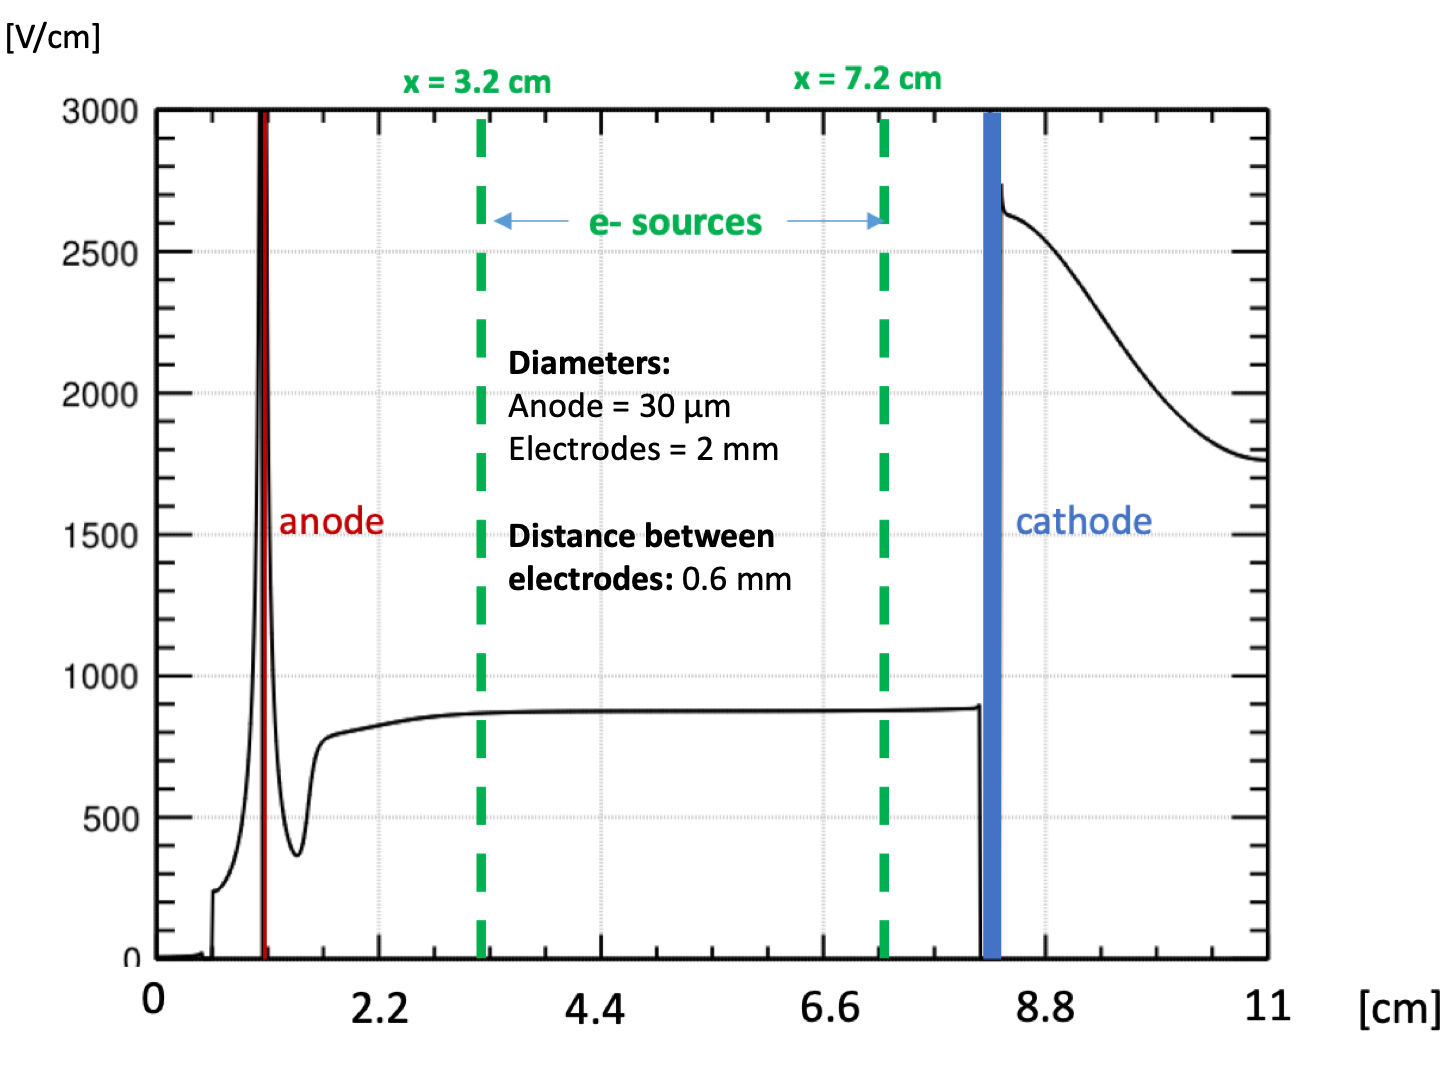
\includegraphics[width=\textwidth]{efield_goodsep.png}
		\caption{Electric field profile with electrode separation of 0.6 mm and diameter of 2 mm.}
		\label{fig:eprof_goodsep}
	\end{subfigure}
	\caption{Simulations electric field profile within the sensitive region of the DMS with various electrode diameters and distances.}
	\label{fig:eprof}
\end{figure}

Lastly, in Fig. \ref{fig:eprof_goodsep}, the electrode diameter was set to 2 mm and the distance between electrodes was decreased to 0.6 mm. The field here in between the sources is nearly homogeneous. Fig. \ref{fig:eprof_goodzoom} is zoomed in to that area between sources to verify how flat ($.i.e.$ homogeneous) the field is there.

Because of these simulations, we were able to identify the frame size, electrode and anode wire diameter, and distances between components. The distance between the cathode and the first set of electrodes was also chosen to be 0.6 mm, which also is the distance from the last electrode to the ground plate.

\subsection{Drift Velocity}
The last step of the Garfield++ simulations is to determine what we should expect for a drift velocity from the DMS. Just like the physical DMS, the drift velocity is calculated by taking the drift times from ionization electrons created at the lines of the sources that travel to the sources. In the simulations, electrons are started at one of the two areas where the sources would exist. From here the simulation tracks them toward the anode, and a histogram of the drift time is filled.

\begin{figure}[h!]
	\centering
	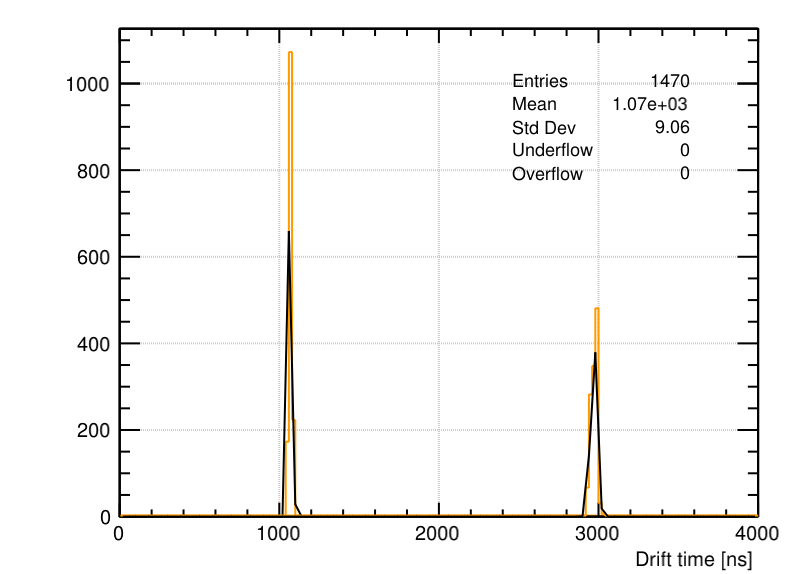
\includegraphics[width=0.8\linewidth]{figures/vdc_sim_td.png}
	\caption{Simulated drift time for electrons beginning at both the near and far sources from the anode.}
	\label{fig:vdc_sim_td}
\end{figure}

Fig. \ref{fig:vdc_sim_td} shows the drift times from 20 ionization electrons beginning at locations of both the sources.  By taking the means from both Gaussian fits of each collection of drift times with the distance between the two sources ($i.e.$ 4 cm), the drift velocity can be calculated. That drift velocity from Garfield++ simulations is
\begin{equation}
v = \frac{\Delta d}{\Delta t} = \frac{d_f - d_n}{t_f - t_n} = \frac{4 \times 10^{4} \mathrm{\mu m}} {2969.90 \mathrm{ ns} - 1070.75 \mathrm{ ns}} = 21.06  \mathrm{ \mu m/ns}.
\end{equation}
This gave us an idea what to expect when beginning the data acquisition process. 